\documentclass{standalone}

\usepackage[dvipsnames]{xcolor}
\usepackage{tikz}

\begin{document}
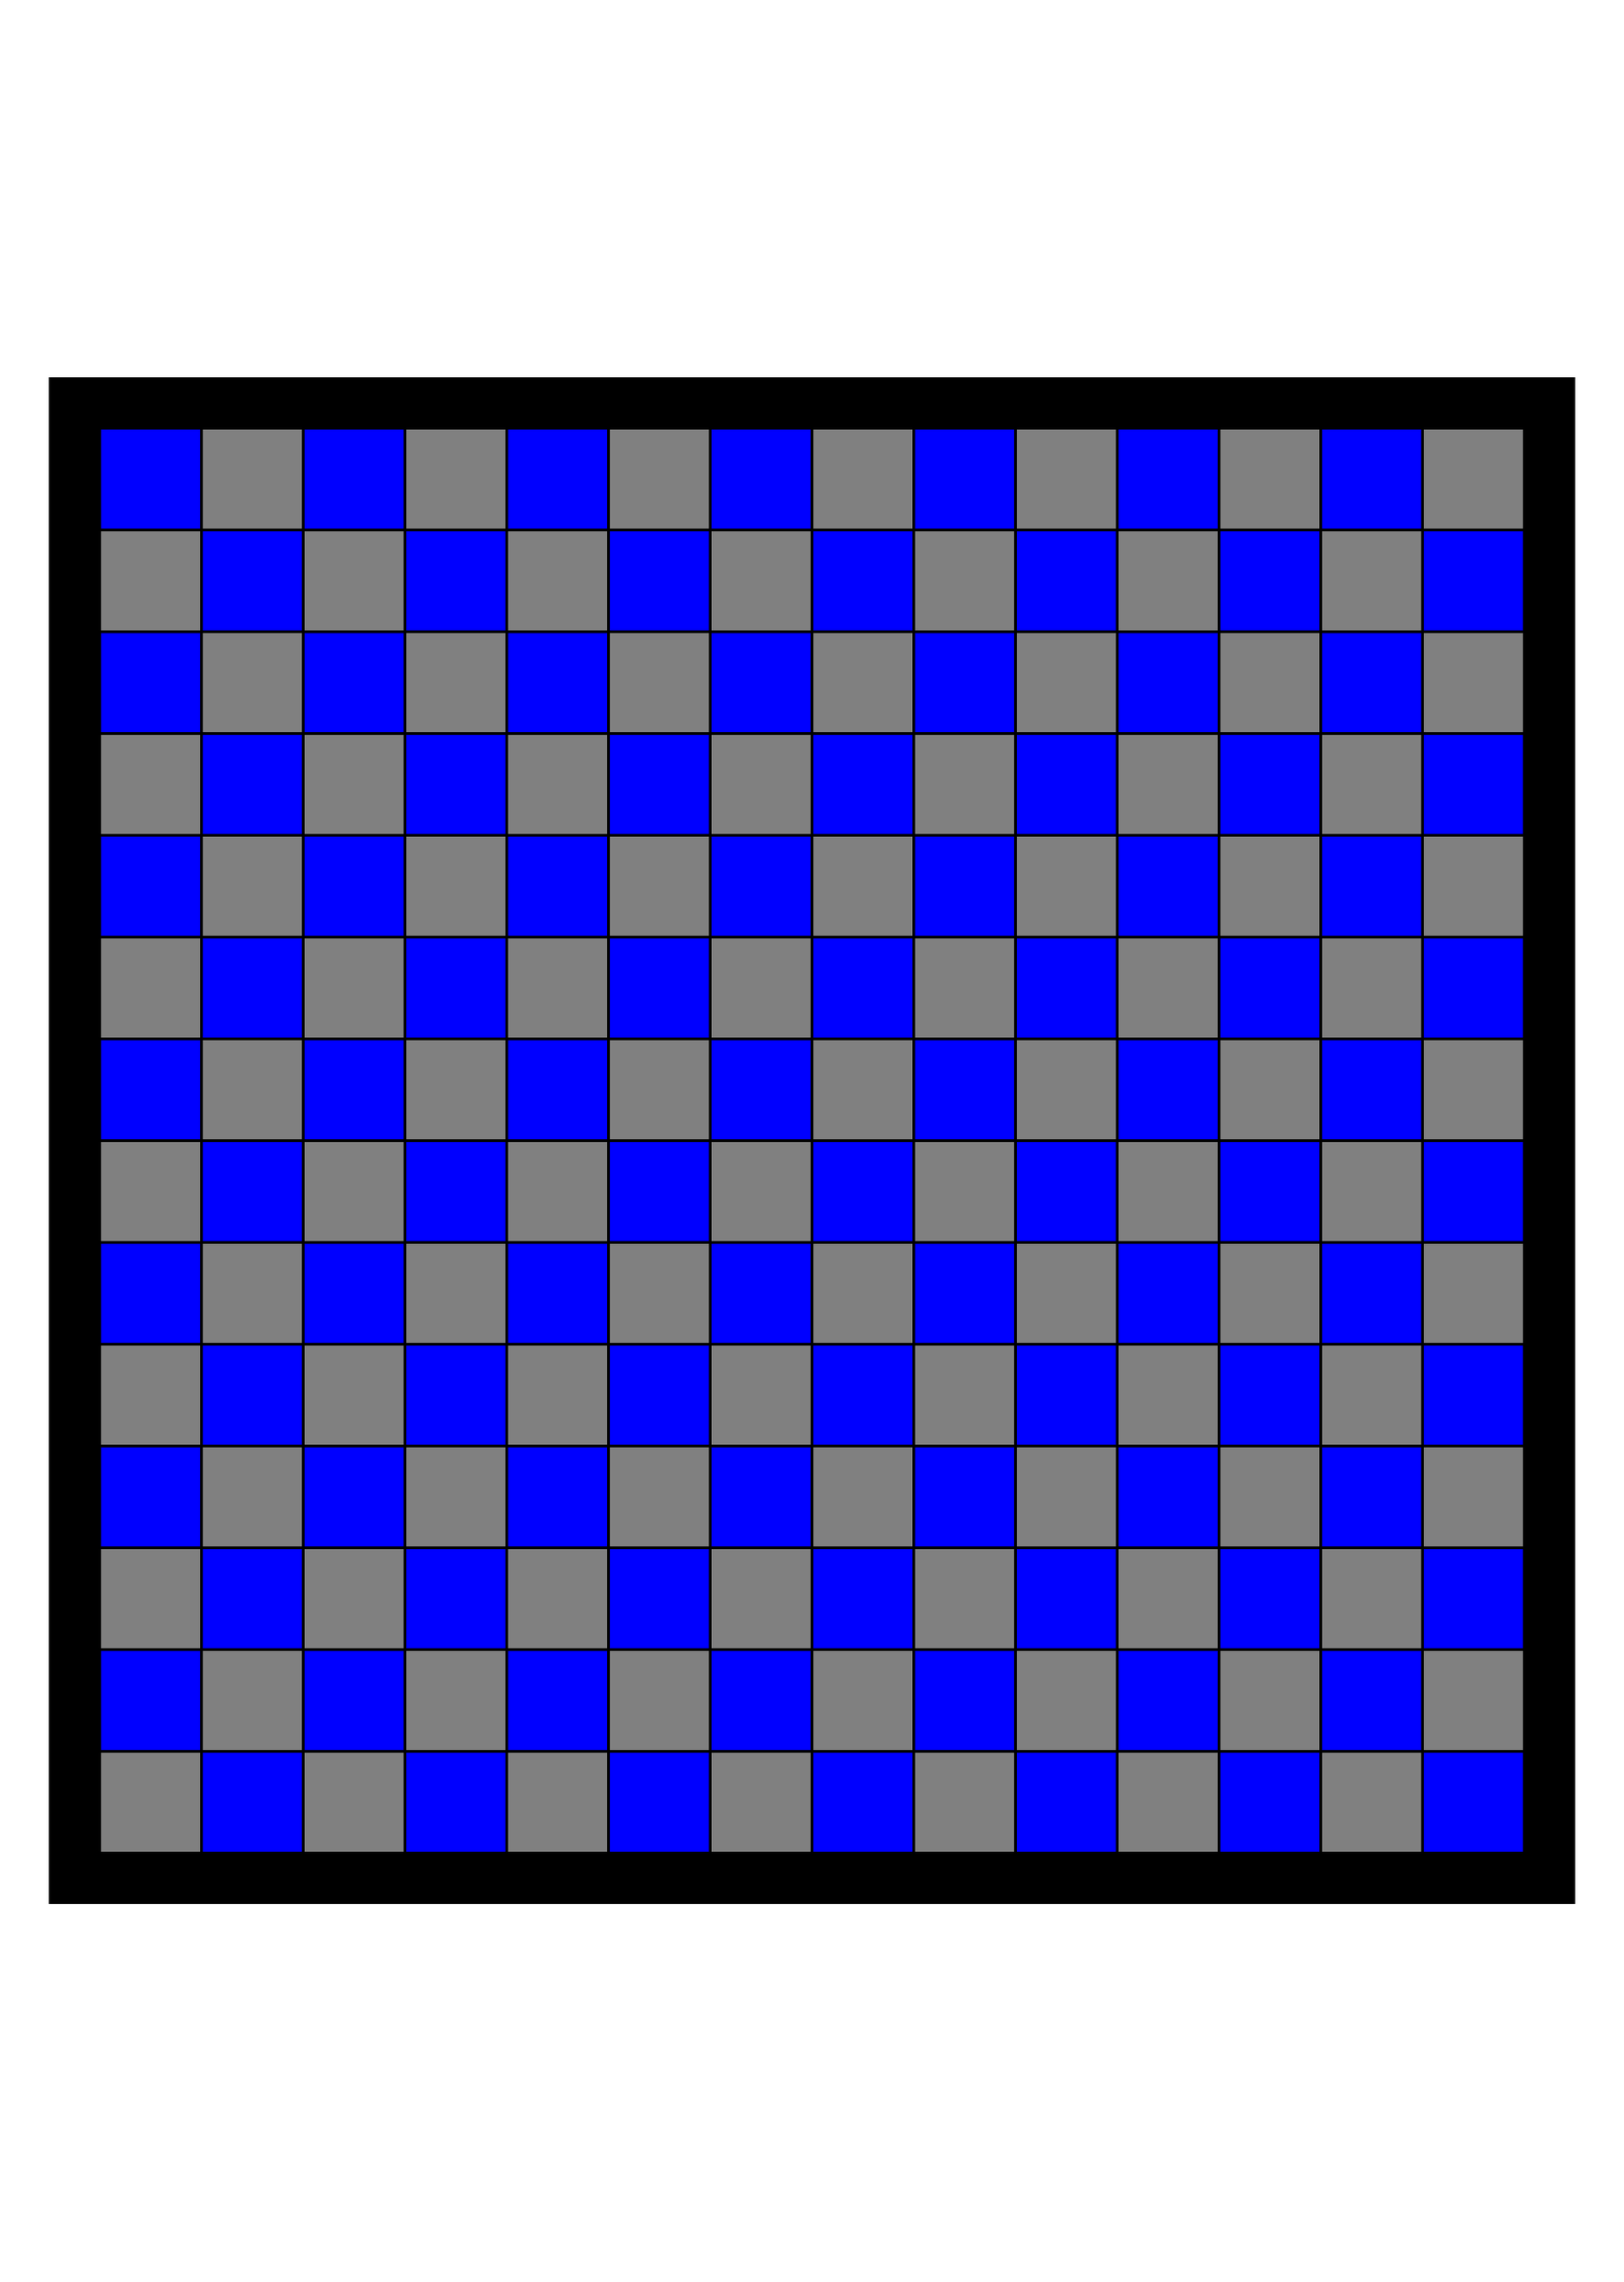
\begin{tikzpicture}

\path (-148.5mm, -210mm) -- (148.5mm, 210mm);
\node[fill=black, minimum height=11.25in, minimum width=11.25in] at (0,0) {};

\foreach \i in {-6.5,-4.5,-2.5,-0.5,1.5,3.5,5.5}
	\foreach \j in {-6.5,-4.5,-2.5,-0.5,1.5,3.5,5.5}
		\node[draw, ultra thick, fill=Gray, minimum width=0.75in, minimum height=0.75in, inner sep=0pt] at (\i*0.75in, \j*0.75in) {};
		
\foreach \i in {-5.5,-3.5,-1.5,0.5,2.5,4.5,6.5}
	\foreach \j in {-6.5,-4.5,-2.5,-0.5,1.5,3.5,5.5}
		\node[draw, ultra thick, fill=Blue, minimum width=0.75in, minimum height=0.75in, inner sep=0pt] at (\i*0.75in, \j*0.75in) {};

\foreach \i in {-5.5,-3.5,-1.5,0.5,2.5,4.5,6.5}
	\foreach \j in {-5.5,-3.5,-1.5,0.5,2.5,4.5,6.5}
		\node[draw, ultra thick, fill=Gray, minimum width=0.75in, minimum height=0.75in, inner sep=0pt] at (\i*0.75in, \j*0.75in) {};
		
\foreach \i in {-6.5,-4.5,-2.5,-0.5,1.5,3.5,5.5}
	\foreach \j in {-5.5,-3.5,-1.5,0.5,2.5,4.5,6.5}
		\node[draw, ultra thick, fill=Blue, minimum width=0.75in, minimum height=0.75in, inner sep=0pt] at (\i*0.75in, \j*0.75in) {};

%\draw (-148.5mm, 148.5mm) -- (148.5mm, 148.5mm);
%\draw (-148.5mm, -148.5mm) -- (148.5mm, -148.5mm);


\end{tikzpicture}
\end{document}